\documentclass{standalone}
\usepackage{tikz}
\usepackage{pgfplots}
\begin{document}
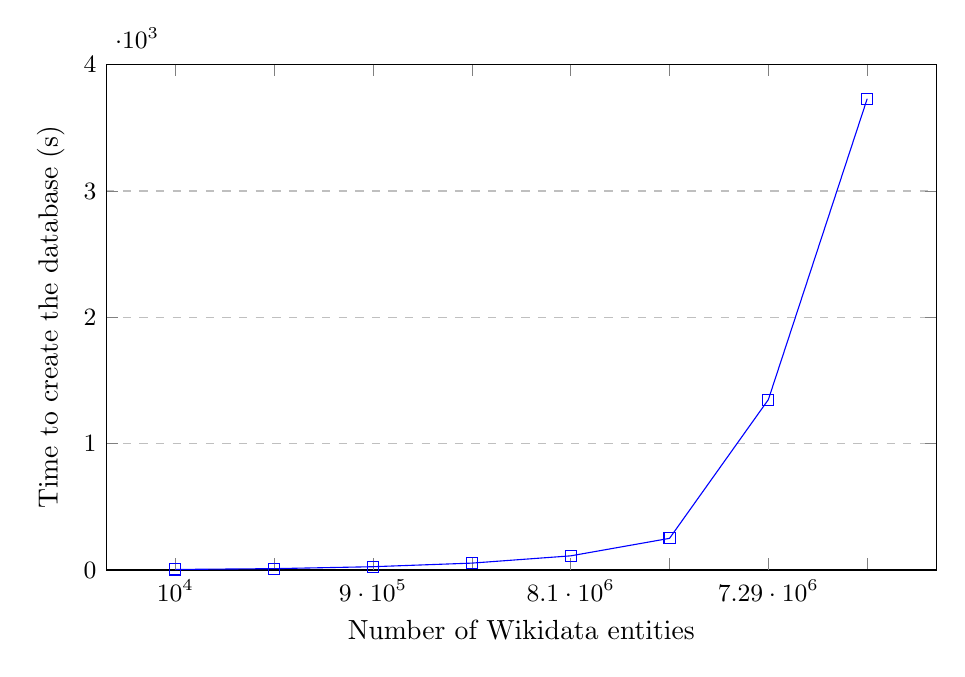
\begin{tikzpicture}
    \begin{axis}[
            title={},
            xlabel={Number of Wikidata entities},
            ylabel={Time to create the database (s)},
            ymin=0, ymax=4000,
            xmode=log,
            xtick=data,
            xticklabel=\empty,
            extra x ticks={10000,90000,810000,7290000},
            extra x tick labels={$10^4$, $9\cdot10^5$, $8.1\cdot10^6$, $7.29\cdot10^6$},
            height=8cm,
            scaled y ticks={base 10:-3},
            width=\textwidth,
            legend pos=north west,
            ymajorgrids=true,
            grid style=dashed,
            tick align=inside,
            every tick label/.append style={font=\small}
        ]
        \addplot[
            color=blue,
            mark=square,
        ]
        coordinates {
                (10000,4.56)
                (30000,11.05)
                (90000,26.36)
                (270000,54.87)
                (810000,112.30)
                (2430000,250.86)
                (7290000,1349.10)
                (21870000,3730.33)
            };
    \end{axis}
\end{tikzpicture}
\end{document}